\documentclass[12pt, letterpaper]{article}
\usepackage{float}
\usepackage{parskip}
\usepackage{graphicx}
\usepackage{amsmath}
\usepackage{amssymb}
\usepackage{setspace}
\usepackage{geometry}
\usepackage{subcaption}
\usepackage{indentfirst}
\usepackage{anyfontsize}
\usepackage[utf8]{inputenc}
\usepackage[american]{babel}
\usepackage[babel]{csquotes}
\usepackage[	style=phys,
				articletitle=false,
				backend=bibtex,
				biblabel=brackets,
				chaptertitle=false,
				pageranges=false]{biblatex}

\addbibresource{physics-ia.bib}
\defbibheading{bibliography}{\section{Bibliography}}
\bibliography{physics-ia}

\geometry{letterpaper, portrait, margin=1in}
\graphicspath{{../imgs/}}

\newcommand{\sorta}[1]{`#1'}
\newcommand{\poses}[1]{#1's}

\title{The Optimal Strength-Retaining Hole Pattern for Sheet Material}
\author{Tynan Purdy}
\date{May 2019}

\begin{document}
\large
\doublespace{}
\parindent=0.5in

{\fontsize{12}{14.4}
  {\singlespace
    \pagenumbering{gobble}
    \maketitle
    \begin{center}
    002129-0004 \\
    \vspace{4mm}
    IB Physics HL IA \\
    \vspace{4mm}
    Words:  \\ % words
    \end{center}
  }
}	

\newpage
\pagenumbering{arabic}

%TC:break Abstract
\begin{abstract}
One of the greatest challenges of structural engineering is to reduce the weight of a system without compromising its strength. Hole patterns are a go-to solution to make parts lighter and maintain the majority of their rigidity. The problem is, what hole pattern is best? With many 2D tessellation patterns to choose from, it can be difficult to determine the optimal pattern to use. This investigation will simulate stresses on test sheet parts with a variety of polygon hole patterns to determine which shape maintains the highest strength in an array of scenarios. 

Words: % words

\end{abstract}
%TC:break _main_

\newpage
\tableofcontents
\newpage

\section{Background}

Sheet metal is one of the most commonly used materials in engineering, but especially finds its place in the field of robotics. Sheet metal provides a stiff, structural component while taking little space and weight. Robotics frequently requires complicated geometry in small volumes. Sometimes sheet metal can be used as a light structural material instead of solid or tube extrusion. In high school competitive robotics, teams use sheet metal to make custom gearboxes, gussets, base-plates, even entire drive-trains. For all of these applications, applying a lightening hole pattern is a great way to reduce weight while maintaining an acceptable durability and stiffness.

\begin{figure}[H]
	\centering
	\label{fig:frc1}
	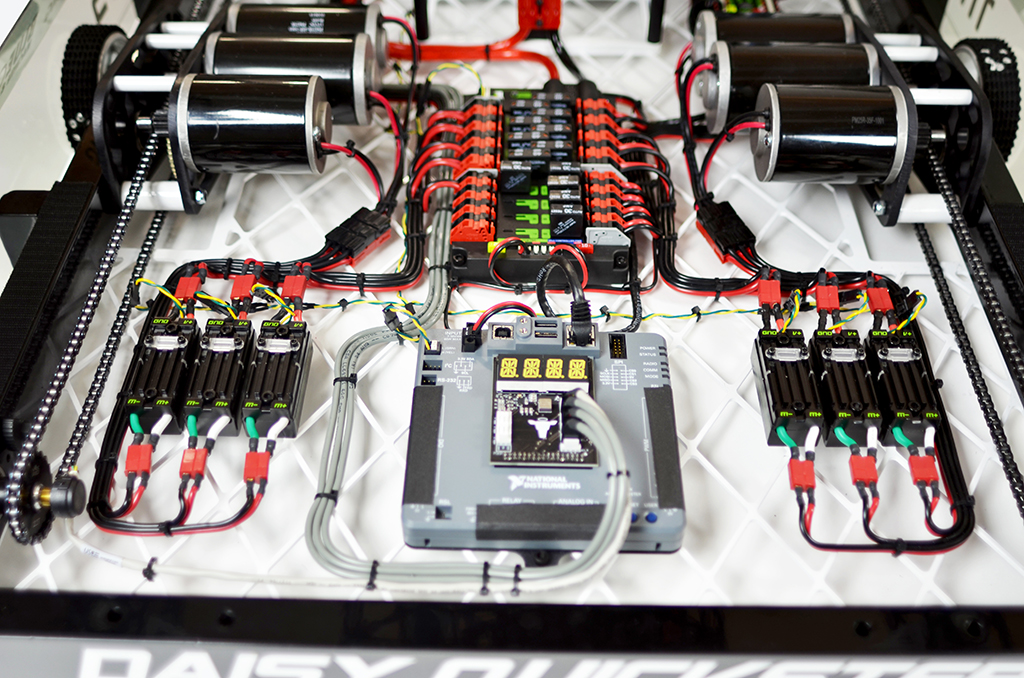
\includegraphics[width=.8\linewidth]{frc-ex1}
	\caption{FIRST Robotics Competition robot (team 1538) with rectangular diamond hole pattern}
\end{figure}

\subsection{Statics}

Statics is an area of physics thoroughly used in engineering, and particularly in the area of solid mechanics and structural engineering. 

\subsection{Solid Mechanics}

The field of solid mechanics analyzes the deformations of a solid under system changes. Deformation is the change ($\Delta$) between the rest shape and the final shape. These changes can include changes in forces, temperature, phase changes and other internal or external changes \autocite{chou_elasticity:_1992}. A variety of models have been developed to describe different types of deformations of solids:



\begin{itemize}
\item Stress: The force applied over a specific cross-sectional area
\item Strain: The response of a system to an applied stress
\item Plasticity: The degree to which an object can deform
\item Elasticity: The degree to which an object can return to rest shape after deformation
\end{itemize}

For this investigation, the elasticity and plasticity model will be used to describe the characterize the simulated deformations. 

\begin{singlespace}
\begin{equation}
	\label{eq:stress}
	\sigma_x \equiv \lim_{\Delta A \rightarrow 0} \frac{\Delta N}{\Delta A}
\end{equation}
\begin{small}
\begin{itemize}
\item[] $\sigma_x =$ stress
\item[] $\Delta N =$ fraction of normal force $N$
\item[] $\Delta A =$ cross-sectional area element
\end{itemize}
\end{small}
\end{singlespace}


\begin{singlespace}
\begin{equation}
	\label{eq:strain}
	\varepsilon_x \equiv \frac{\sigma_x}{E} + \alpha \Delta T
\end{equation}
\begin{small}
\begin{itemize}
\item[] $\varepsilon_x =$ strain
\item[] $\sigma_x =$ stress
\item[] $E =$ modulus of elasticity
\item[] $\alpha =$ temperature coefficient
\item[] $\Delta T =$ change of temperature
\end{itemize}
\end{small}
\end{singlespace}

\section{Simulation}

\subsection{Variables}



To keep the stress analysis of each part fair, certain properties were controlled for every part. 

\begin{itemize}
\item All parts have the dimensions of 1000mm x 1000mm x 5mm
\item All parts are set to the material 6061 Aluminum Alloy
\item All parts have a mass of 2.525kg, within $\pm2.5\%$ error (except the solid test part)
\item All parts have a 10mm perimeter with no holes
\item All polygon holes have a 10mm wide edge
\item An equal force will be applied to each part for each test
\end{itemize}

Each part is not exactly 2.5kg because the skill in SolidWorks and time required to reach that target are beyond the scope of this investigation and the researcher. 2.5kg was chosen as the target mass because it was the approximate mass of the \sorta{square-pattern} part. The 10mm perimeter was included to ensure equal mass where forces will be applied in the various simulations, and that the parts would have a closed perimeter. 

Variables that will change based on the shape used, and be recorded, are as follows:

\begin{itemize}
\item Hole Area
\item Part Surface Area
\item Number of holes
\end{itemize}

A total of 6 different patterns will be tested in simulated stress tests.

\begin{enumerate}
\item Filled (control)
\item Square
\item Square Diamond
\item Hex
\item Hex Diamond
\item Triangle
\end{enumerate}

The \sorta{filled} pattern is a solid sheet. It is used as a reference test as well as a data point to show stress properties when no holes are used. It should be noted that not all holes have the same area since hole patterns that do not match the shape of the part will not fit an integer number of shapes, and some shapes will be \sorta{cut off}. The vertices of incomplete shapes are not identical to the vertices of whole holes. The inconsistent vertices may have an effect on the results of the investigation. The surface area of each part is the 2D surface area of the flat sheet. 

\begin{figure}[H]
	\label{parts}
	\caption{Test Parts}
	\begin{subfigure}[b]{.3\linewidth}
		
\includegraphics[width=\linewidth]{filled}
		\caption{Filled}
	\end{subfigure}
	\begin{subfigure}[b]{.3\linewidth}
		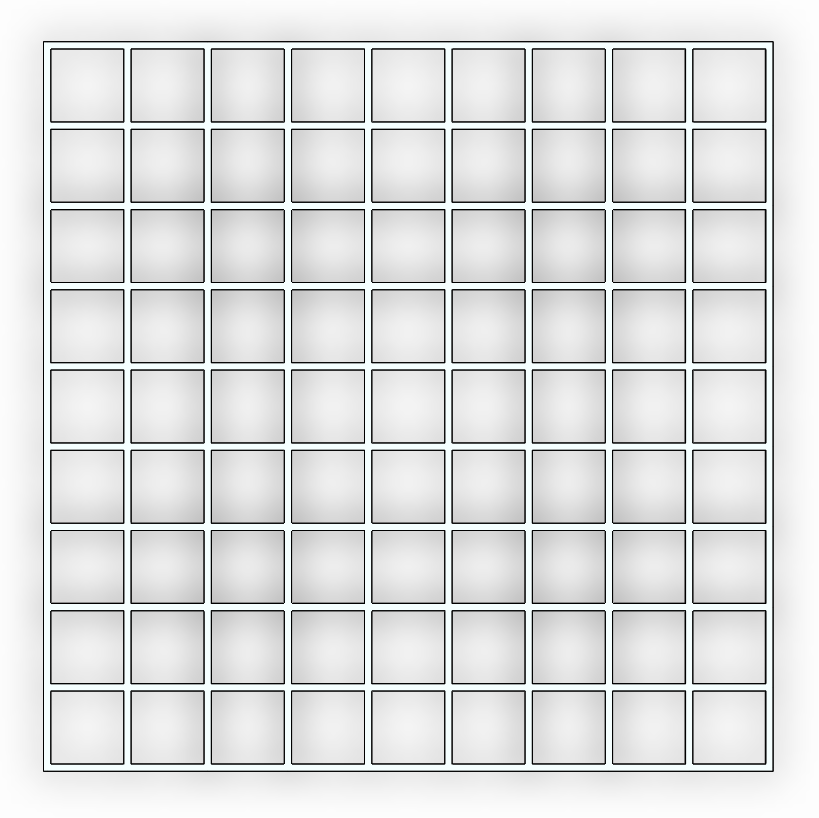
\includegraphics[width=\linewidth]{square}
		\caption{Square}
	\end{subfigure}
	\begin{subfigure}[b]{.3\linewidth}
		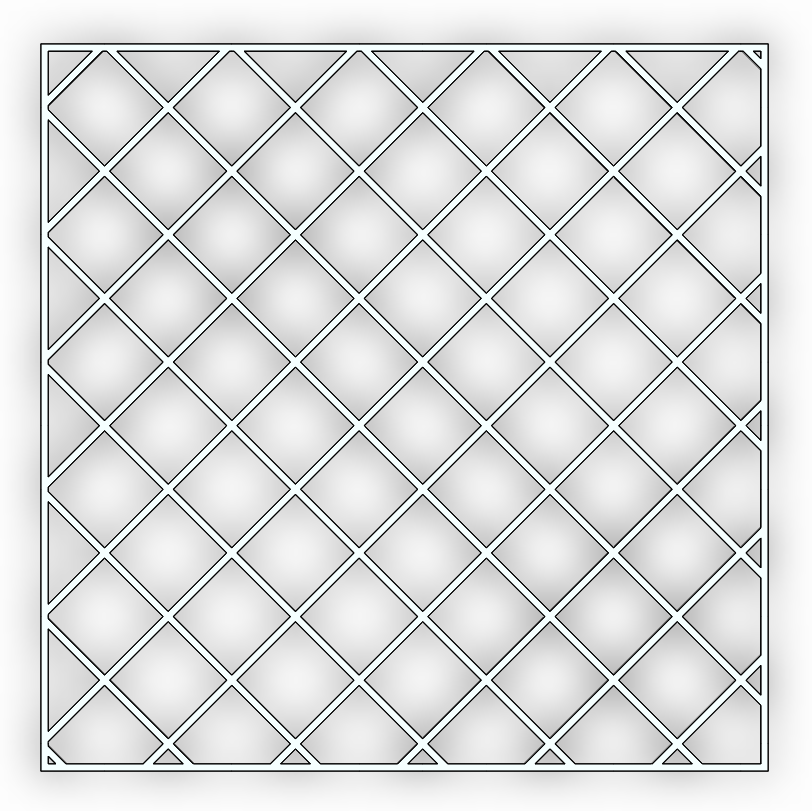
\includegraphics[width=\linewidth]{square-diamond}
		\caption{Square Diamond}
	\end{subfigure}
	\begin{subfigure}[b]{.3\linewidth}
		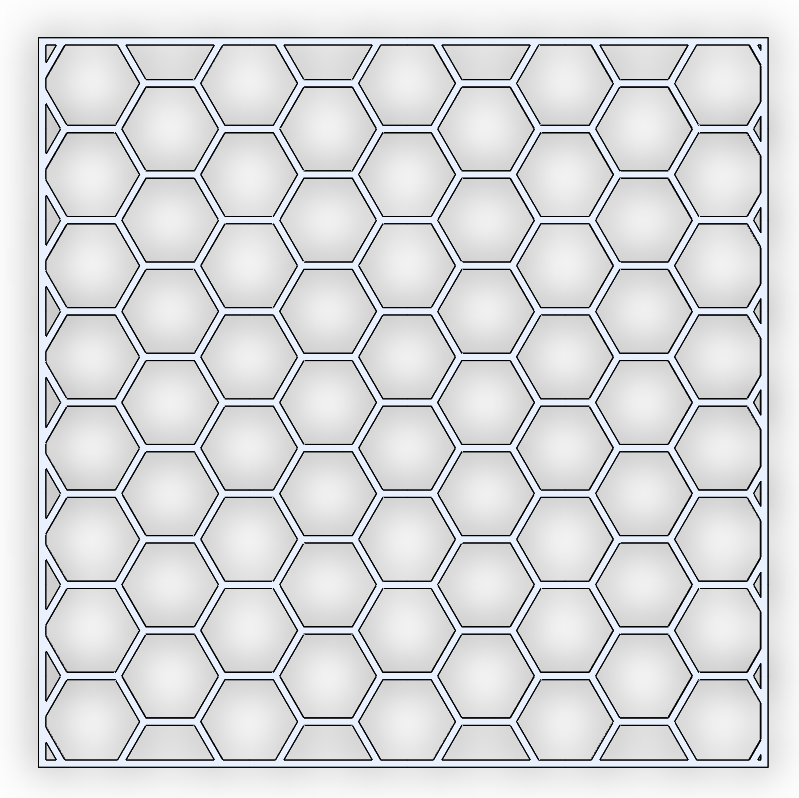
\includegraphics[width=\linewidth]{hex}
		\caption{Hex}
	\end{subfigure}
	\begin{subfigure}[b]{.3\linewidth}
		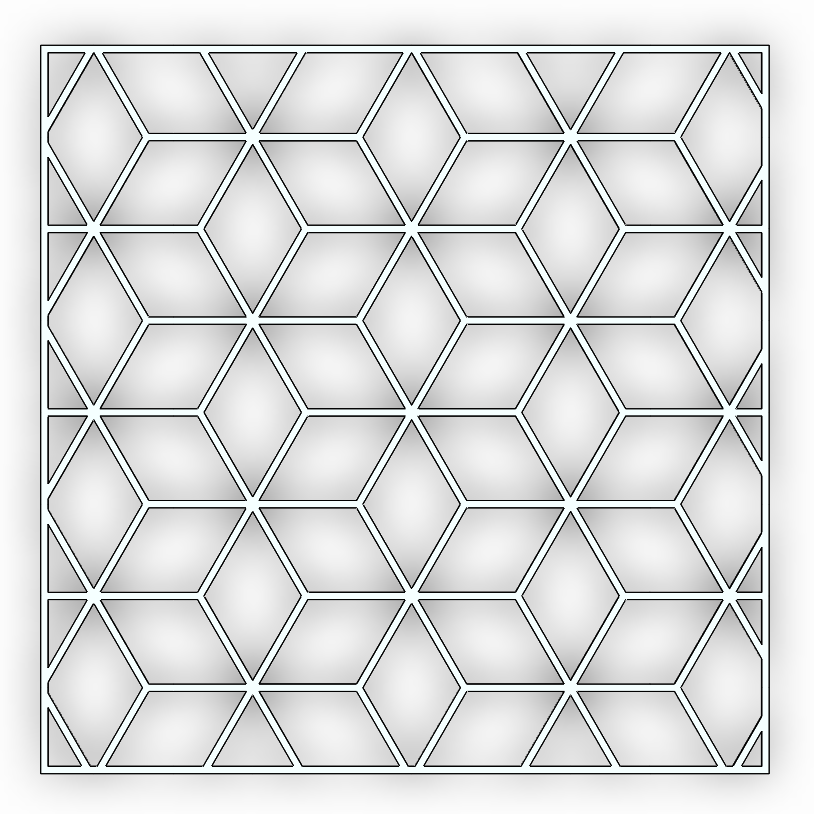
\includegraphics[width=\linewidth]{hex-diamond}
		\caption{Hex Diamond}
	\end{subfigure}
	\begin{subfigure}[b]{.3\linewidth}
		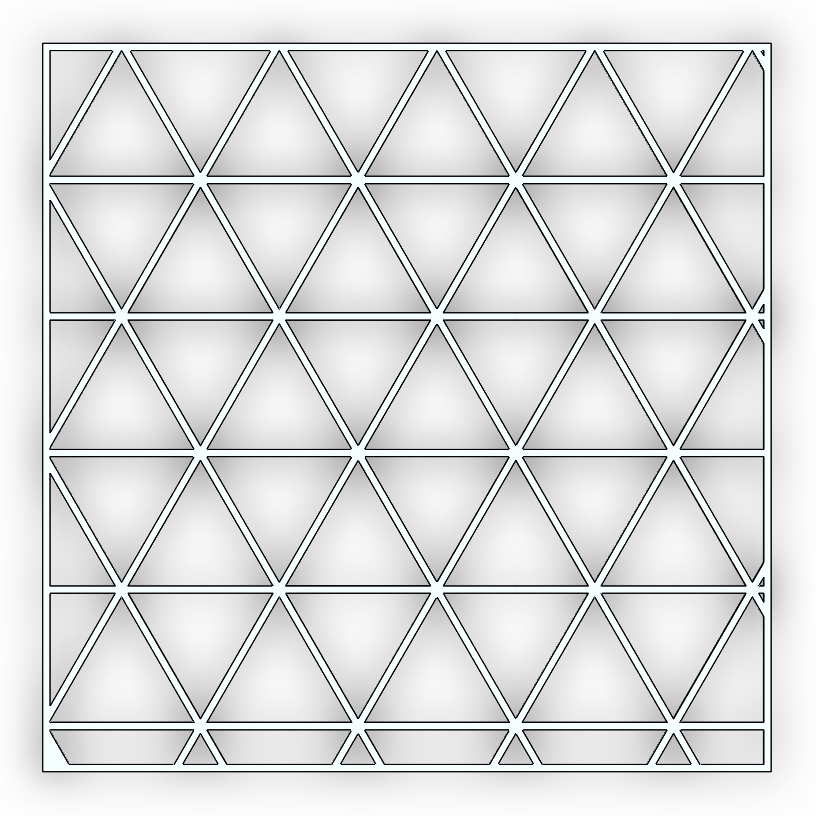
\includegraphics[width=\linewidth]{triangle}
		\caption{Triangle}
	\end{subfigure}
	\begin{subfigure}[b]{\linewidth}
	\begingroup
	\setlength{\tabcolsep}{10pt} % Default value: 6pt
	\renewcommand{\arraystretch}{1.5} % Default value: 1
		\begin{tabular}{ | c | c | c | c | c | }\hline
			Pattern 			& Mass (kg) 	& Surface Area (m$^2$)	& Max Hole Area (cm$^2$) 	& $n$ Holes 	\\\hline
			Filled				& 13.50 		& 1.000 						& 0			 					& 0			\\\hline
			Square			& 2.565 		& 0.190 						& 100.00		 					& 81			\\\hline
			Square Diamond	& 2.545 		& 0.188 						& 129.37	 						& 62.77		\\\hline
			Hex				& 2.506 		& 0.186 						& 114.55	 						& 71.06		\\\hline
			Hex Diamond		& 2.497 		& 0.185 						& 155.38	 						& 52.45		\\\hline
			Triangle			& 2.500 		& 0.185						& 170.65				 			& 47.76		\\\hline
		\end{tabular}
		\caption{Part Properties}
	\endgroup
	\end{subfigure}
\end{figure}

\subsection{Procedure}

A series of stress simulations will be performed on each of the 6 test parts. 

\begin{enumerate}
\item Linear Tension
\item Linear Compression
\item Torsion
\item Bending
\end{enumerate}

\section{Analysis}

\section{Conclusion}

\newpage
\printbibliography{}

\newpage
\section{Appendix}
\listoffigures{}

\end{document}